\documentclass{article}
\usepackage[a4paper, total={6in, 9in}]{geometry}
\usepackage{graphicx}
\usepackage{xcolor}
\usepackage{listings}
\definecolor{vgreen}{RGB}{104,180,104}
\definecolor{vblue}{RGB}{49,49,255}
\lstset{
    language=Verilog,
    % wrap text
    breaklines=true, 
    % line numbers
    numbers=left,
    numberstyle=\tiny\color{black},
    numbersep=10pt,
    % other styling
    basicstyle=\small\ttfamily,
    keywordstyle=\color{vblue},
    identifierstyle=\color{black},
    commentstyle=\color{vgreen},
    tabsize=2
}
\graphicspath{ {../Images/} }

\title{
    \begin{large}
        ELEC374 - Lab 2
    \end{large}
}
\author{Naod Dereje - 20103501, Thierry Jones - 20108349, Jamie Won - 20113217}

\begin{document}
\maketitle
\cleardoublepage
\tableofcontents
\cleardoublepage


\section{Components}
    The purpose of this lab was to design, simulate, implement and verify a simple RISC computer(Mini SRC), including the circuits associated with the logic behind: 
    Select and Encode, Memory Subsystem, CON FF and Input/Output ports. Verilog was chosen over VHDL as it is better for more complex simulations. The verilog code 
    for each of these components can be found in the Appendices.
    
    \subsection{Select and Encode}


    \subsection{Memory Subsystem}
    

    \subsection{CON FF}
    

    \subsection{Input/Output Ports}

\section{Circuitry Demonstration}
    To demonstrate the success of the RAM and memory interface logic, multiple testbenches were created to simulate each operation. 
    The testbenches all have their own control sequences unique to every operation and can be found in the appendices. The following subsections 
    of the cicuitry demonstration will detail the changes made in the test benches due to the control sequence changing as well as the waveforms generated by each simulation.
    Each instruction used to demonstrate the circuitry requires a specific OP Code. The following table shows the OP Code values stored in RAM initially, their address in RAM and also the instruction itself. For a full version of the initial RAM state, please see Appendix \ref{ram_init}.
    \begin{figure}[h!] \label{relevant_ram_init}
        \begin{center}
            \begin{tabular}{|c|c|c|}
                \hline
                Address (hex) & Instruction & Op code (hex) \\
                \hline
                1* & st \$90, R1 & 10080090 \\ % Thierry, Naod, don't change this line, see below figure for rationale
                \hline
                1* & st \$90(R1), R1 & 10080090 \\ % Thierry, Naod, don't change this line, see below figure for rationale
                \hline
                ? & addi R2, R1, \$-5 & 590FFFFB \\
                \hline
                ? & andi R2, R1, \$26 & 61080026 \\
                \hline
                ? & ori R2, R1, \$26 & 69080026 \\
                \hline
                20 & brzr R2, 35 & 91000023 \\
                \hline
                21 & brnz R2, 35 & 91200023 \\
                \hline
                22 & brpl R2, 35 & 91400023 \\
                \hline
                23 & brmi R2, 35 & 91600023 \\
                \hline
                18 & jal R1 & A0800000 \\ % Thierry, Naod, don't change this line, these are the jump instructions - we don't want to generate new waveforms
                \hline
                19 & jr R1 & 98800000 \\ % Thierry, Naod, don't change this line, these are the jump instructions - we don't want to generate new waveforms
                \hline
            \end{tabular}
            \caption{Table of relevant values in RAM initially}
        \end{center}
    \end{figure}
    \\
    \small{*Note that these instructions were tested before the rest, thus, the .hex file hadn't be completed. Thus, Appendix \ref{ram_st_case_1} and Appendix \ref{ram_st_case_2} have empty values in RAM where the OP Codes are for later tests.}

    \subsection{Store Instructions}
        Two store instructions were used to test the RAM and memory interface logic. The instruction sequence for \emph{st \$90, R1} and \emph{st \$90(R1), R1} can be found in Appendix \ref{st_case_1_sequence} and Appendix \ref{st_case_2_sequence} respectively. It should be noted that the value $85_{16}$ was preloaded into R1 for both instructions. The specific opcodes for these instructions can be found in Figure \ref{relevant_ram_init}. 
        
        \subsubsection{st \$90, R1}
            This instruction is similar to the load immediate instruction. It is however, in a sense, reversed. Where the load ends by reading from the Z\_LO register and its contents to the specified register, this instruction finishes by reading from the MDR and writing to the RAM. The results of this instruction, in RAM, can be found in Appendix \ref{ram_st_case_1} at address $90_{16}$ (line 22). The following image shows the waveform generated by running this sequence. 

            \begin{figure}[h!]
                \begin{center}
                    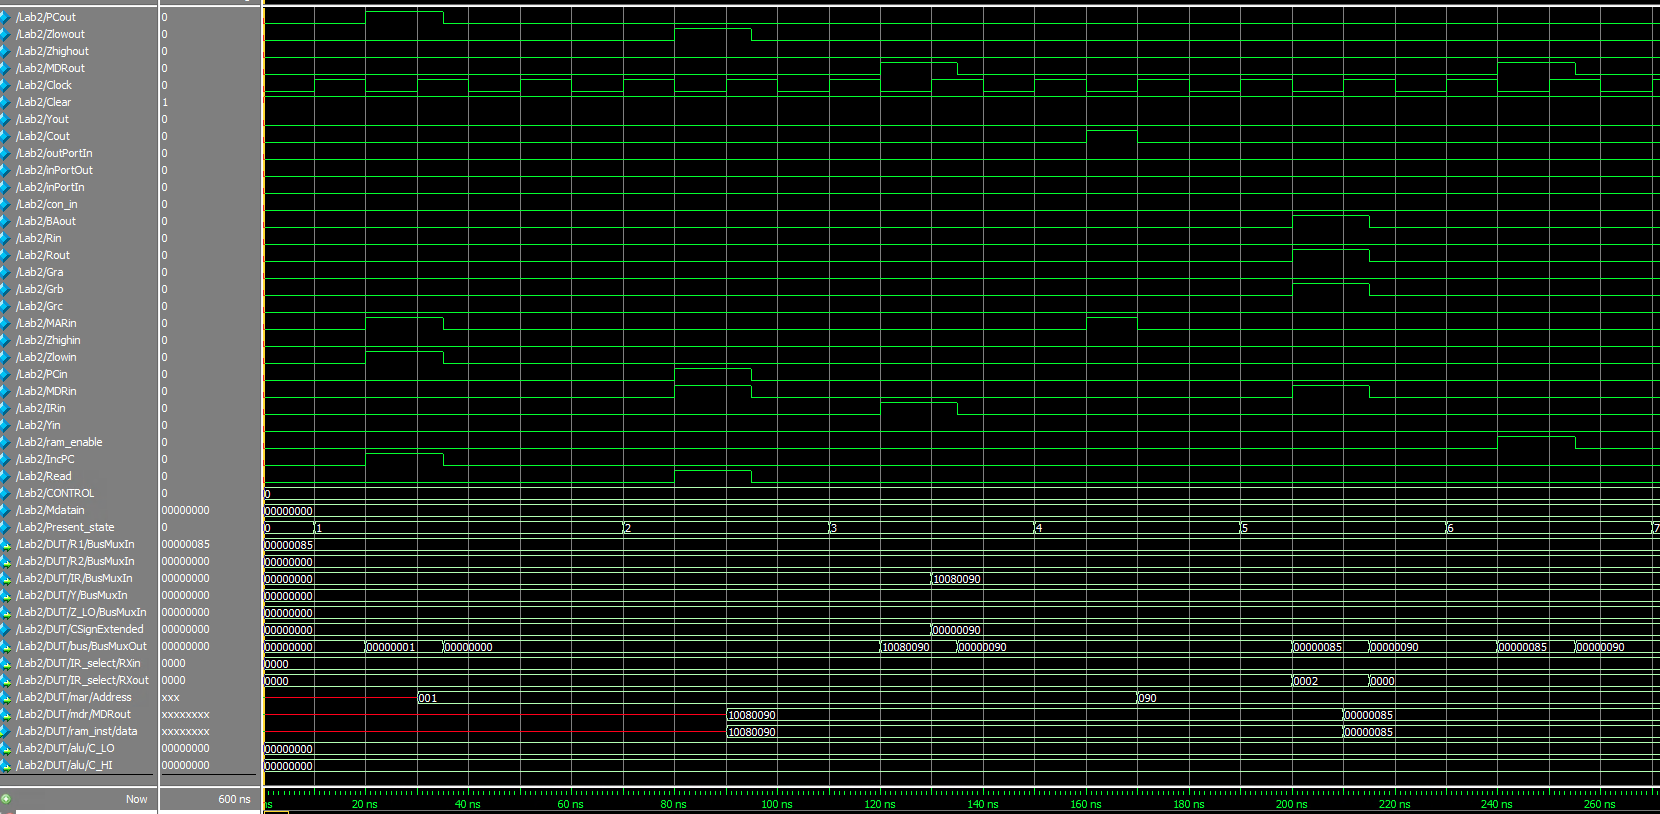
\includegraphics[width=15cm]{st_case_1_wave.png}
                    \caption{A screenshot of the simulated waveforms for the and st \$90, R1 instruction}
                \end{center}
            \end{figure}

        \subsubsection{st \$90(R1), R1}
            This instruction is similar to the load instruction. It is however, in a sense, reversed. While both instructions end by reading from the MDR register, the load instruction writes its contents to the specified register, while the store instruction writes to the RAM. The results of this instruction, in RAM, can be found in Appendix \ref{ram_st_case_2} at address $115_{16}$ (line 38).The following image shows the waveform generated by running this sequence. 

            \begin{figure}[h!]
                \begin{center}
                    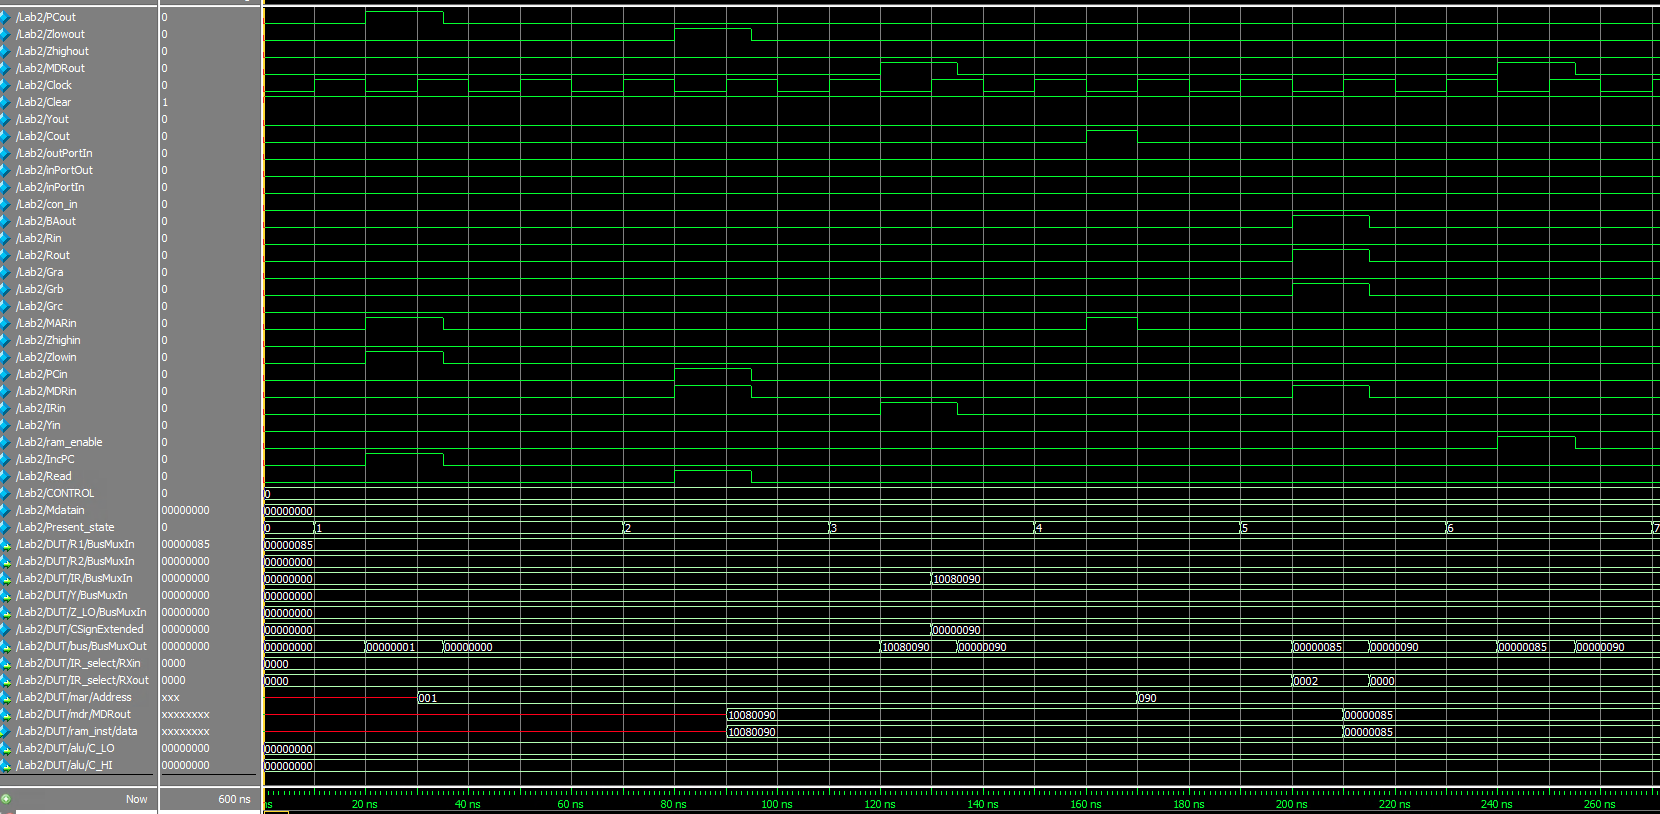
\includegraphics[width=15cm]{st_case_1_wave.png}
                    \caption{A screenshot of the simulated waveforms for the and st \$90(R1), R1 instruction}
                \end{center}
            \end{figure}
            

    \subsection{ALU Immediate Instructions}
        The ALU immediate instruction functionality was simulating using the \emph{addi R2, R1, -5}, \emph{andi R2, R1, \$26} and \emph{ori R2, R1, \$26} instructions. The instruction sequences can be found in Appendix \ref{addi_sequence}, Appendix \ref{andi_sequence} and Appendix \ref{ori_sequence} respectively. The instructions sequences for these sections differ only in the control signal used for the ALU and the preloaded instruction in RAM. The specific opcodes for these instructions can be found in Figure \ref{relevant_ram_init}. Otherwise, the sequences follow the guidelines given in the spec document exactly.

    \subsection{Branch Instructions}
        Four branch instructions were used to test the RAM and \emph{con_ff} module. The instruction sequences \emph{brzr R2, 35}, \emph{brnz R2, 35}, \emph{brpl R2, 35} and \emph{brmi R2, 35} can be found in Appendix \ref{brzr_sequence}, \ref{brnz_sequence}, \ref{brpl_sequence} and \ref{brmi_sequence} respectively. The specific opcodes for these instructions can be found in Figure \ref{relevant_ram_init}. The value of R2 will be preloaded with the decimal value 1 for each of the simulated waveforms. 

        \subsubsection{brzr R2, 35}
            Since the value $1_{10}$ was preloaded into R2, and $1 \neq 0$ it is expected that the PC does not jump in T6, or when the Present\_State signal is equal to 7. This is reflected in the image below.

                \begin{figure}[h!]
                    \begin{center}
                        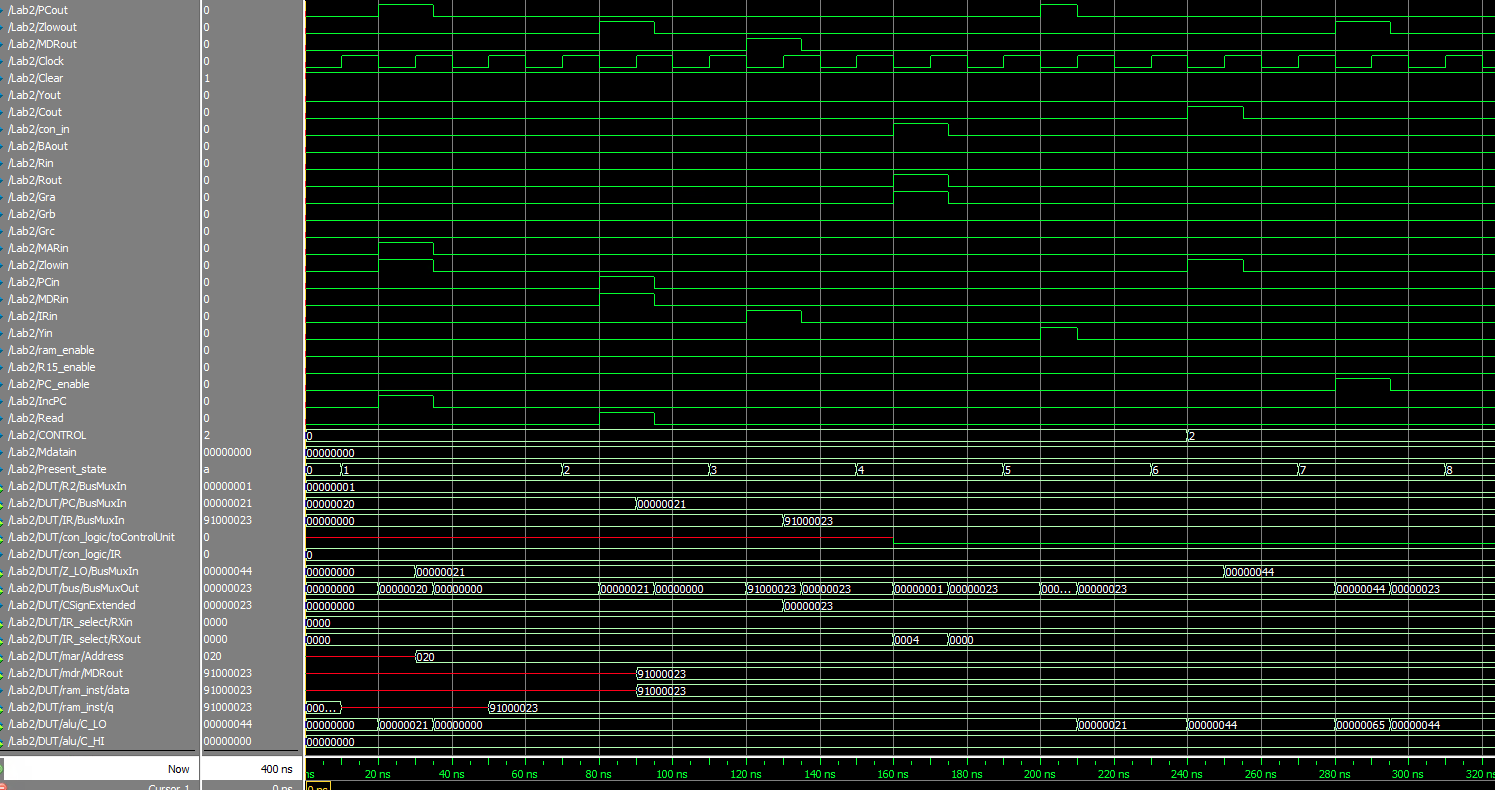
\includegraphics[width=15cm]{brzr_wave.png}
                        \caption{A screenshot of the simulated waveforms for brzr, brzr R2, 35}
                    \end{center}
                \end{figure}

        \subsubsection{brnz R2, 35}
            Since the value $1_{10}$ was preloaded into R2, and $1 \neq 0$ it is expected that the PC jumps in T6, or when the Present\_State signal is equal to 7. This is reflected in the image below. It should be noted that $21_{16} + 1_{10} + 35_{10} = 45_{16}$. 

                \begin{figure}[h!]
                    \begin{center}
                        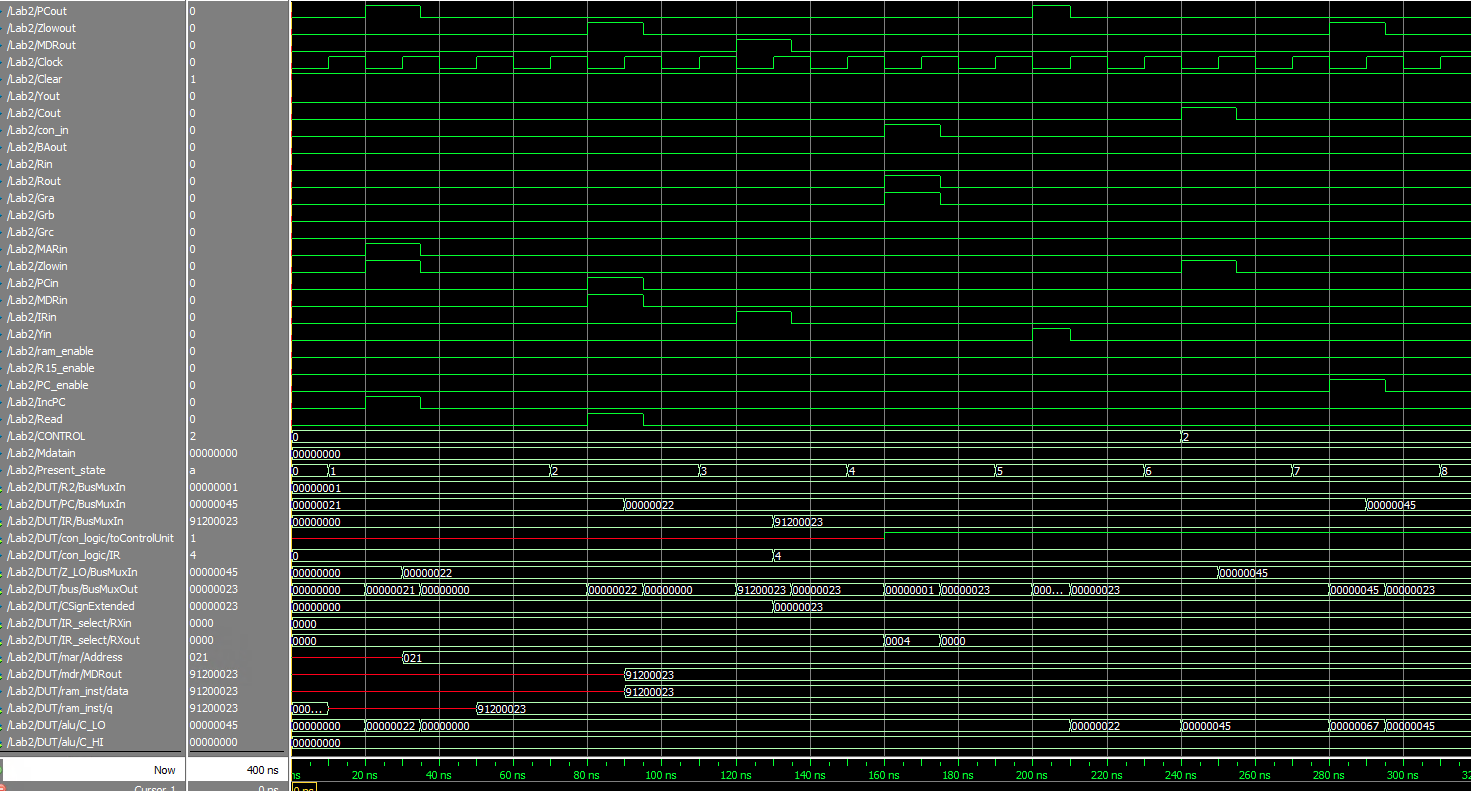
\includegraphics[width=15cm]{brnz_wave.png}
                        \caption{A screenshot of the simulated waveforms for brnz, brnz R2, 35}
                    \end{center}
                \end{figure}

        \subsubsection{brpl R2, 35}
            Since the value $1_{10}$ was preloaded into R2, and $1 > 0$ it is expected that the PC jumps in T6, or when the Present\_State signal is equal to 7. This is reflected in the image below. It should be noted that $22_{16} + 1_{10} + 35_{10} = 46_{16}$. 
        
                \begin{figure}[h!]
                    \begin{center}
                        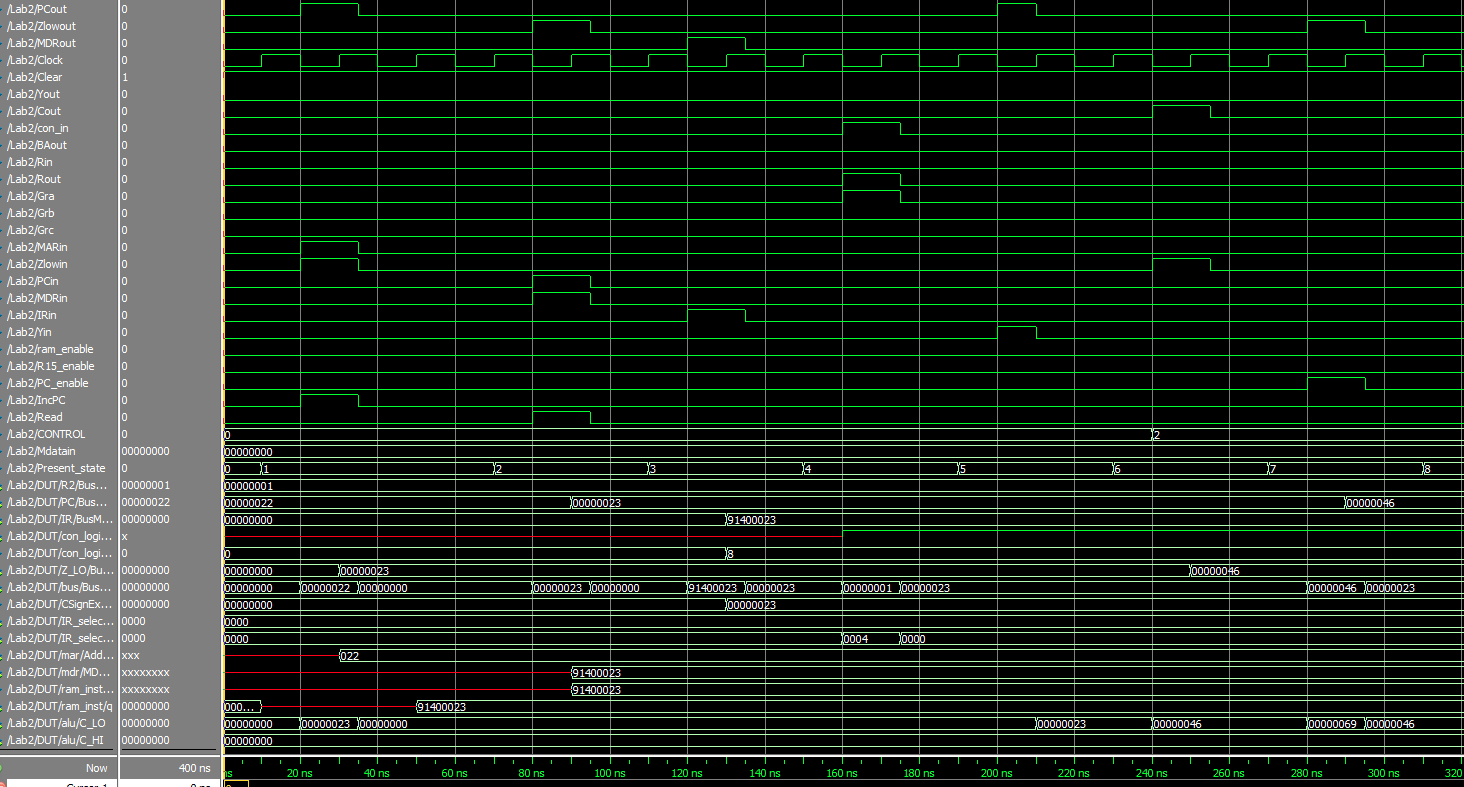
\includegraphics[width=15cm]{brpl_wave.png}
                        \caption{A screenshot of the simulated waveforms for brpl, brpl R2, 35}
                    \end{center}
                \end{figure}

        \subsubsection{brmi R2, 35}
            Since the value $1_{10}$ was preloaded into R2, and $1 > 0$ it is expected that the PC does not jump in T6, or when the Present\_State signal is equal to 7. This is reflected in the image below.
        
                \begin{figure}[h!]
                    \begin{center}
                        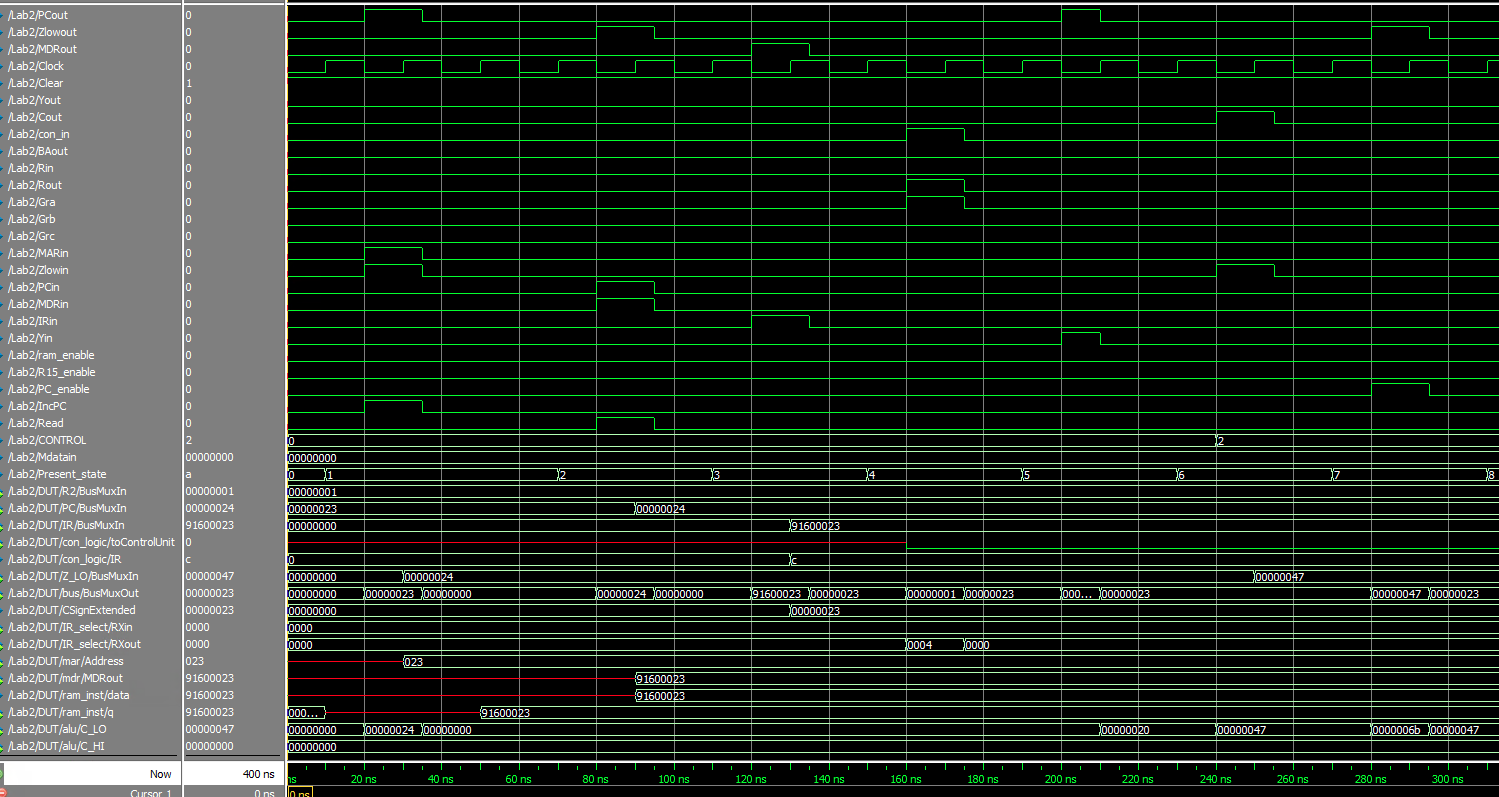
\includegraphics[width=15cm]{brmi_wave.png}
                        \caption{A screenshot of the simulated waveforms for brmi, brmi R2, 35}
                    \end{center}
                \end{figure}

    \subsection{Special Instructions}
    The special instructions functionality was simulated using the \emph{mfhi R2} and \emph{mflo R2} commands. For the most part, they were identical to the template provided for the ALU immediate instructions. The difference lay in T3, where instead of \emph{Rout} being enabled, \emph{Rin} was and the \emph{highout} and \emph{lowout} signals were enabled for the \emph{mfhi R2} and \emph{mflo R2} commands respectively. 
    
        \subsubsection{mfhi R2}
            The HI register was preloaded to have a value of 100. As seen in T3, or when the signal Present\_state is equal to 4, the value stored in R2 is set to the value in HI. It should be noted that $100_{10}$ is equivalent to $64_{16}$. The control sequence for this instruction can be found in Appendix \ref{mfhi_sequence}.

        \subsubsection{mflo R2}
            The LO register was preloaded to have a value of 10. As seen in T3, or when the signal Present\_state is equal to 4, the value stored in R2 is set to the value in LO. It should be noted that $10_{10}$ is equivalent to $a_{16}$. The control sequence for this instruction can be found in Appendix \ref{mflo_sequence}.
      


\appendix
\section{Select and Encode}
\section{Memory Subsystem}
\section{CON FF}
\section{Input/Output Ports}
The input and output ports in the datapath allow for the bus to receive values from an input unit, as well as output values from the bus onto the output unit. In a real implmentation of an I/O port instruction, the logic for these ports would be used to read from some input given to port, and give feedback to the system through some output such as updated the result of an arithmetic instruction, or the bit pattern after a bit shift or rotation was completed.
\section{Control Sequences}
    \subsection{st \$90, R1} \label{st_case_1_sequence}
    \subsection{st \$90(R1), R1} \label{st_case_2_sequence}
    \subsection{brzr R2, 35} \label{brzr_sequence}
    \subsection{brnz R2, 35} \label{brnz_sequence}
    \subsection{brpl R2, 35} \label{brpl_sequence}
    \subsection{brmi R2, 35} \label{brmi_sequence}
    \subsection{addi R2, R1, -5} \label{addi_sequence}
    \subsection{andi R2, R1 \$26} \label{andi_sequence}
    \subsection{ori R2, R1 \$26} \label{ori_sequence}
    \subsection{mfhi R2} \label{mfhi_sequence}
    \subsection{mflo R2} \label{mflo_sequence}
\section{RAM}
    \subsection{Initial Contents} \label{ram_init}
    \subsection{Post "st" instructions}
        \subsubsection{st \$90, R1} \label{ram_st_case_1}
            \lstinputlisting{../memory_data/st_case_1_memdata.txt}
        \subsubsection{st \$90(R1), R1} \label{ram_st_case_2}
            \lstinputlisting{../memory_data/st_case_2_memdata.txt}


\end{document}
